\capitulo{4}{Técnicas, herramientas y componentes}

Esta parte de la memoria tiene como objetivo presentar las técnicas metodológicas y las herramientas de desarrollo que se han utilizado para llevar a cabo el proyecto. Si se han estudiado diferentes alternativas de metodologías, herramientas, bibliotecas se puede hacer un resumen de los aspectos más destacados de cada alternativa, incluyendo comparativas entre las distintas opciones y una justificación de las elecciones realizadas. 
No se pretende que este apartado se convierta en un capítulo de un libro dedicado a cada una de las alternativas, sino comentar los aspectos más destacados de cada opción, con un repaso somero a los fundamentos esenciales y referencias bibliográficas para que el lector pueda ampliar su conocimiento sobre el tema.

\section{Web Scraping}
Es una técnica utilizada para extraer información de una página web utilizando las etiquetas de que dispone el propio lenguaje interpretado de HTML (del inglés <<HyperText Markup Language>> o lenguaje de marcas de hipertexto) para organizar elementos dentro de una página web, de forma que se introduce dentro de una etiqueta y subetiquetas hasta llegar al contenido del elemento requerido. Podemos entenderlo como si fueran contenedores lógicos configurables.
En nuestro caso, podremos utilizarlo desde Python sirviéndonos de la librería <<beautifulsoup>> siempre que necesitemos obtener información de una página web.

\section{Tirada de cable con guía pasacables}
El procedimiento a seguir es el siguiente:
\begin{enumerate}
        \item Se abren las tapas de dos cajas de derivación próximas.
        \item Se introduce una guía pasacables (herramienta plástica con la forma de cuerda para introducir cables por canalizaciones) por el extremo de uno de los tubos dentro de la caja hasta llegar al otro extremo.
        \item Se asegura el cable a uno de los extremos de la guía pasacables.
        \item Se tira del otro extremo de la guía pasacables hasta conseguir sacar el cable por éste.
\end{enumerate}

\section{RaspberryPi}
En nuestro proyecto tendremos el control de la instalación domótica desde una Raspberry Pi. 
Para dar un enfoque muy general, podemos decir que las placas RaspberryPi son microordenadores que disponen de poca potencia si las comparamos con equipos usuales, pero disponen de suficiente potencia para llevar a cabo este tipo de proyectos.

Se diseñaron en su origen por la RaspBerry Pi Foundation en el Reino Unido para dotar de equipos informáticos a los centros de estudios a un bajo coste, pero el proyecto ha evolucionado para poder desarrollar, además, otras muchas tareas como puede ser nuestro caso, que la utilizaremos como ‘núcleo’ de toda nuestra instalación domótica y, será donde configuremos todo el entorno domótico de la vivienda.
Estas placas pueden ejecutar con agilidad distribuciones Linux y, desde sus distribuciones podemos interactuar con sus famosos “GPIO”, ver imagen \ref{Img:Especificaciones RBP2B}

\begin{figure}
    \centering
    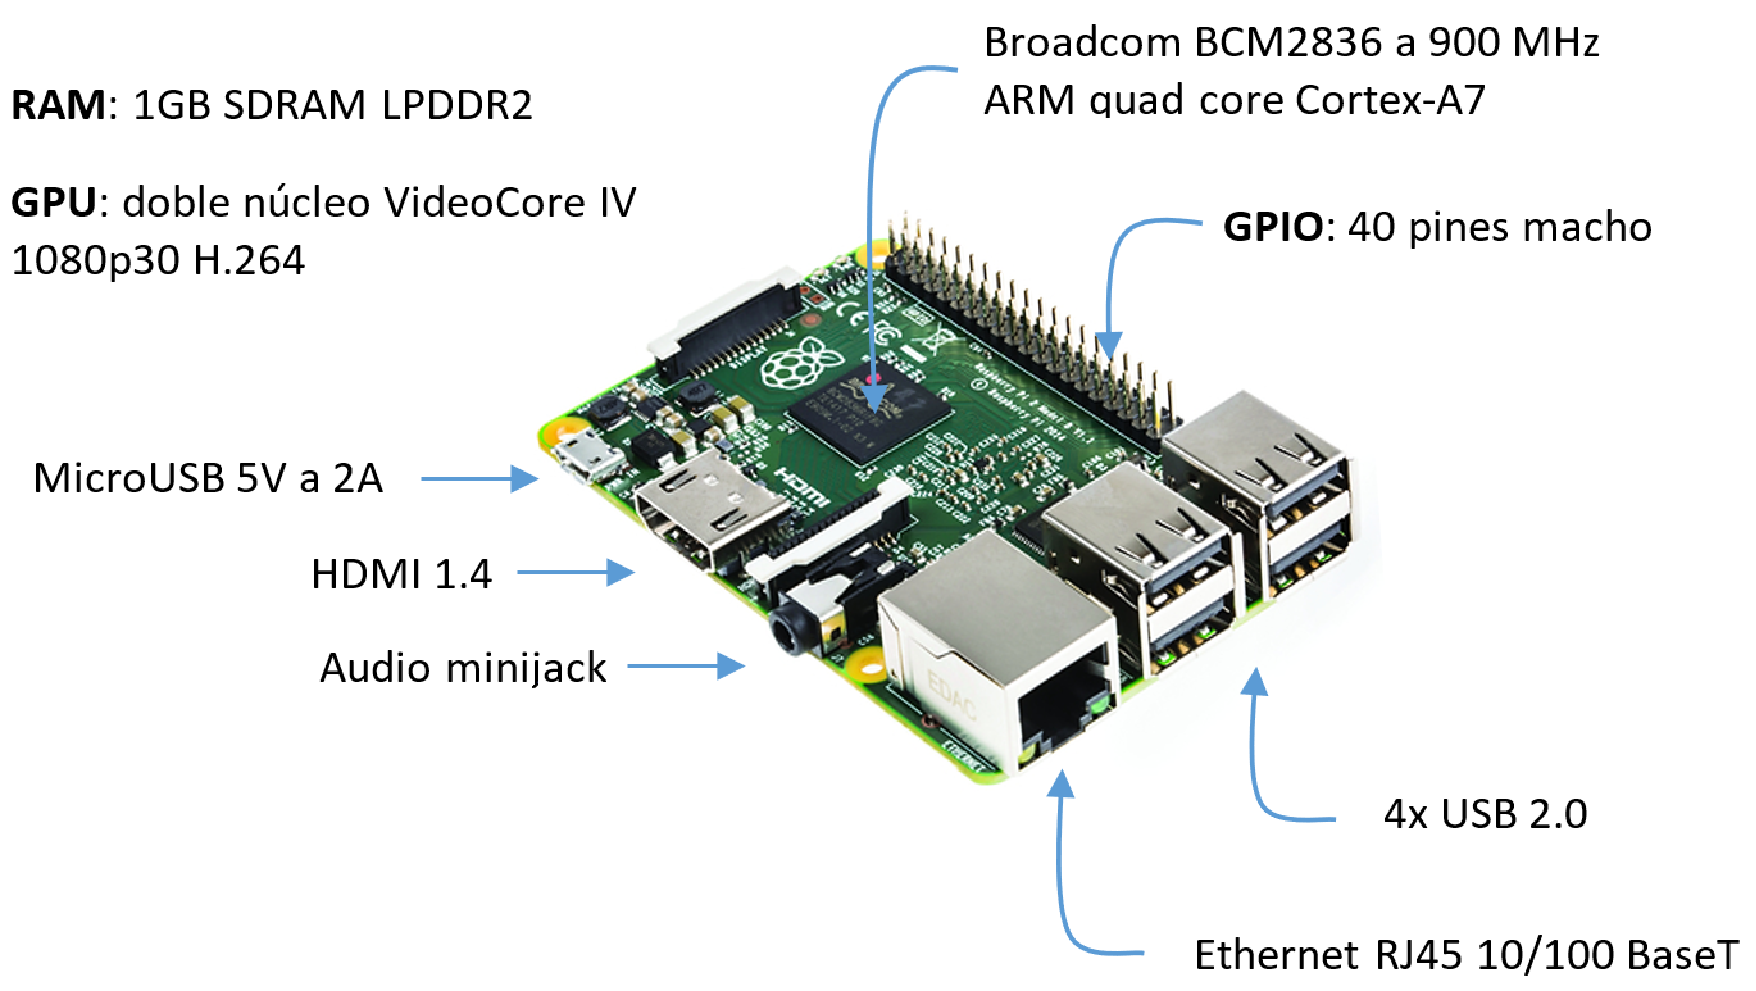
\includegraphics[width=\textwidth]{img/RBP2B.pdf}
    \caption{Especificaciones de Raspberry Pi 2B. Imagen de \url{https://raspberryparatorpes.net} modificada por mí\cite{wiki:Creative}. }\label{Img:Especificaciones RBP2B}
\end{figure}

\section{Relé}
Es un dispositivo electromagnético que desempeña la misma función de un interruptor, es decir, con nuestros relés, dejaremos pasar la energía eléctrica, o no, a nuestros dispositivos. Los relés se activan mediante impulsos eléctricos que abren o cierran el circuito según se predisponga. Podemos verlo en la imagen \ref{Img:Rele1}.
\begin{figure}
    \centering
    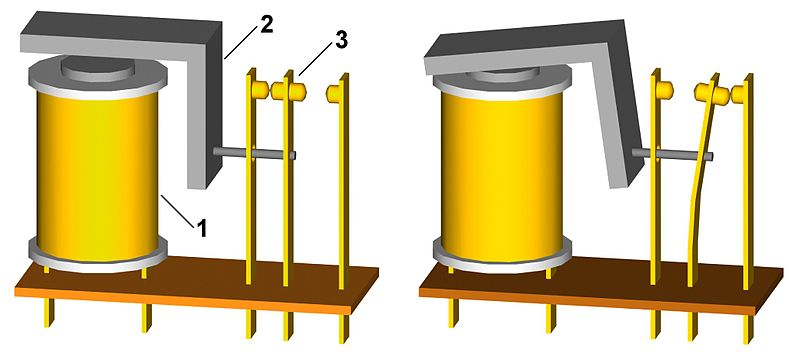
\includegraphics[width=\textwidth]{img/Rele_1.jpg}
    \caption{Estructura interna de un relé. Imagen de \url{https://https://commons.wikimedia.org/}\cite{manual:GNU}}. \label{Img:Rele1}
\end{figure}

\section{Distribución Linux (Raspbian)}
Como he comentado anteriormente, pretendo correr una distribución Linux en nuestro microPc. Las placas Raspberry Pi disponen de unas distribuciones de Linux desarrolladas expresamente para su hardware desde la Raspberry Pi Foundation. De esta manera conseguimos que el entorno esté diseñado para el hardware donde será ejecutado incluyendo, además, utilidades preinstaladas para explotarlas más fácil y eficientemente. Una de estas distribuciones optimizadas y orientadas a estas placas es Raspbian\cite{misc:RbPWeb} o Raspberry Pi OS, que incluye software orientado a la educación, programación y otras de uso general. Algunas de estas aplicaciones son Python\cite{misc:Python} (Lenguaje de programación que pretende que se desarrolle cógigo de una forma sencilla, rápida, poco costosa y legible), Scratch\cite{misc:Scratch}(Simulador amigable para aprender programación.) o Java\cite{misc:Java}(Lenguaje de programación multiplataforma que utiliza una máquina virtual transparente para el usuario para ejecutarse), entre otros.

\section{Placa de Pruebas o ProtoBoard}
Es un tablero electrónico para realizar pruebas. Protoboard es la agrupación de los términos ingleses “prototype board”.
Esta protoboard la he instalado para poder hacer fácilmente el interconexionado entre los cables que llegan de los relés y los que van a la Raspberry Pi, evitando posibles tirones y movimiento de cables a la hora de hacer alguna manipulación.

Éstas, disponen de tres zonas diferenciadas(Ver imagen \ref{Img:Protoboard}):

\begin{itemize}
    \item \textbf{Canal Central}: Está situada en el medio de la placa y es donde se colocan los circuitos.
    \item \textbf{Buses}: Se sitúan en los extremos de la placa y disponen de dos líneas:
    \item \textbf{Línea roja}: Bus positivo o de voltaje.
    \item \textbf{Línea azul}: Bus negativo o de tierra.
    \item \textbf{Pistas}: Se sitúan en la zona central de la placa y, conducen en sentido contrario de las líneas rojas y azul.
\end{itemize}

\begin{figure}
    \centering
    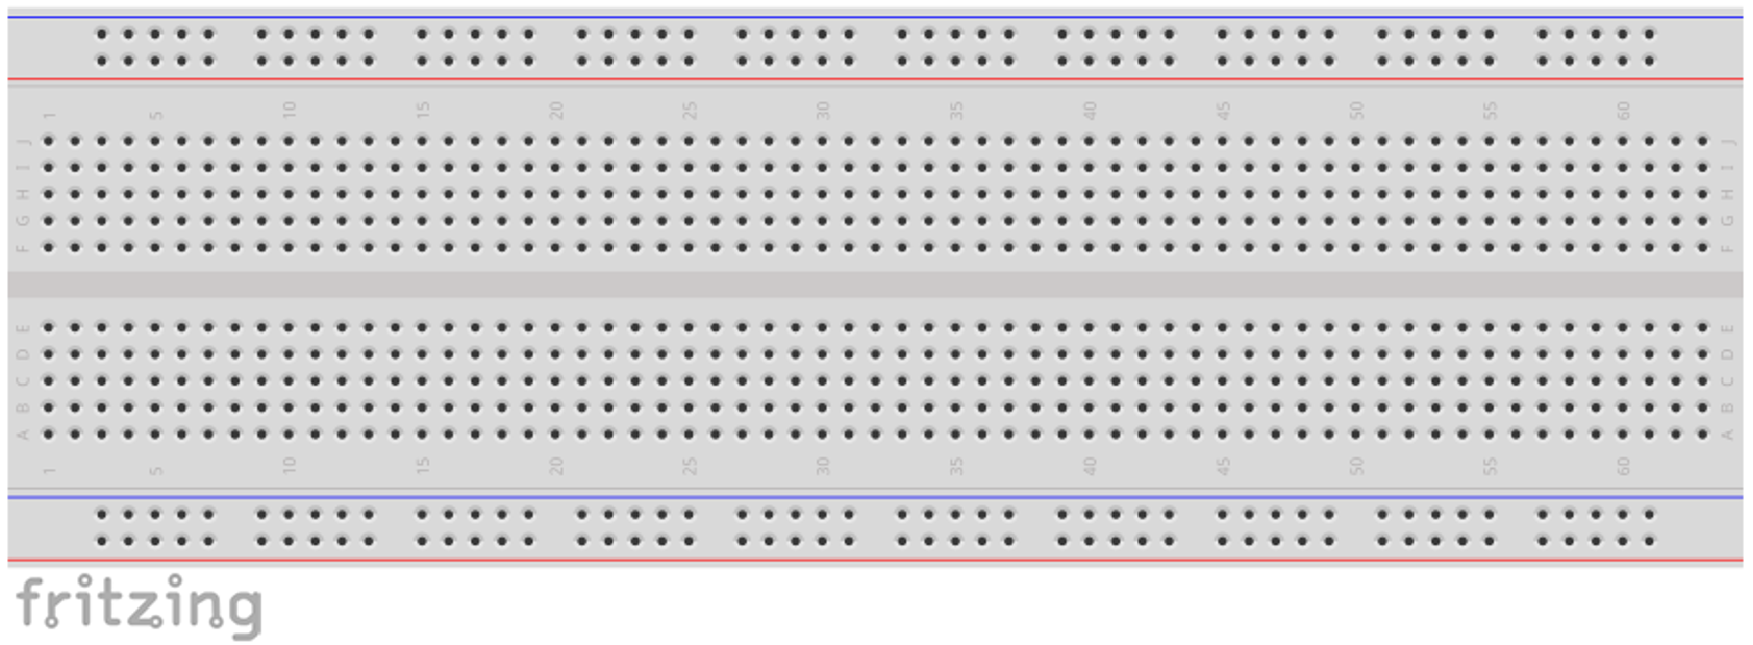
\includegraphics[width=0.9\textwidth]{img/protoboard.pdf}
    \caption{Imagen de una placa <<protoboard>>. } \label{Img:Protoboard}
\end{figure}

\section{Router}
Es un dispositivo que nos permite interconectar diferentes redes de datos. En mi caso dispongo de un router con WiFi integrado para poder dotar a la Raspberry Pi de salida a Internet.



\section{Imágenes}

Se pueden incluir imágenes con los comandos standard de \LaTeX, pero esta plantilla dispone de comandos propios como por ejemplo el siguiente:

\imagen{escudoInfor}{Autómata para una expresión vacía}



\section{Listas de items}

Existen tres posibilidades:

\begin{itemize}
	\item primer item.
	\item segundo item.
\end{itemize}

\begin{enumerate}
	\item primer item.
	\item segundo item.
\end{enumerate}

\begin{description}
	\item[Primer item] más información sobre el primer item.
	\item[Segundo item] más información sobre el segundo item.
\end{description}
	
\begin{itemize}
\item 
\end{itemize}

\section{Tablas}

Igualmente se pueden usar los comandos específicos de \LaTeX o bien usar alguno de los comandos de la plantilla.

\tablaSmall{Herramientas y tecnologías utilizadas en cada parte del proyecto}{l c c c c}{herramientasportipodeuso}
{ \multicolumn{1}{l}{Herramientas} & App AngularJS & API REST & BD & Memoria \\}{ 
HTML5 & X & & &\\
CSS3 & X & & &\\
BOOTSTRAP & X & & &\\
JavaScript & X & & &\\
AngularJS & X & & &\\
Bower & X & & &\\
PHP & & X & &\\
Karma + Jasmine & X & & &\\
Slim framework & & X & &\\
Idiorm & & X & &\\
Composer & & X & &\\
JSON & X & X & &\\
PhpStorm & X & X & &\\
MySQL & & & X &\\
PhpMyAdmin & & & X &\\
Git + BitBucket & X & X & X & X\\
Mik\TeX{} & & & & X\\
\TeX{}Maker & & & & X\\
Astah & & & & X\\
Balsamiq Mockups & X & & &\\
VersionOne & X & X & X & X\\
} 